\subsection{Lead- and Lag compensators}
    \begin{align*}
        C_{\text{lead/lag}} = \frac{\frac{s}{a} + 1}{\frac{s}{b} + 1} = \frac{b}{a} \frac{s+a}{s+b}, \varphi_{\text{max}} = 2 \arctan\left(\sqrt{\frac{b}{a}}\right) - 90^{\circ}\\
        \text{Magnitude in- / decrease } (\omega >> 1): |C(j \omega)| = \pm 20 dB
    \end{align*}
    
    \titel{Lead-Controller}
        \begin{minipage}{0.49\linewidth}
            \begin{align*}
                0 < a < b
            \end{align*}
            Use: increase phase margin\\
            – $k \cdot \sqrt{ab}$: desired crossover frequency\\
            – $\frac{b}{a}$: use for desired phase increase\\
        \end{minipage}
        \begin{minipage}{0.49\linewidth}
            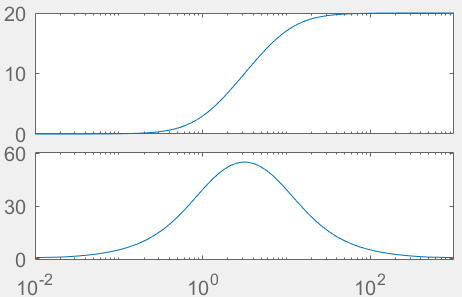
\includegraphics[width = \linewidth]{src/images/lead-controller.png}
        \end{minipage}

    \titel{Lag-Controller}
    \begin{minipage}{0.49\linewidth}
        \begin{align*}
            0 < b < a
        \end{align*}
        Use: improve command tracking / disturbance rejection\\
        To achieve this: multiply $k$ with $\frac{a}{b}$ and choose $a$ big enough not to affect crosover
    \end{minipage}
    \begin{minipage}{0.49\linewidth}
        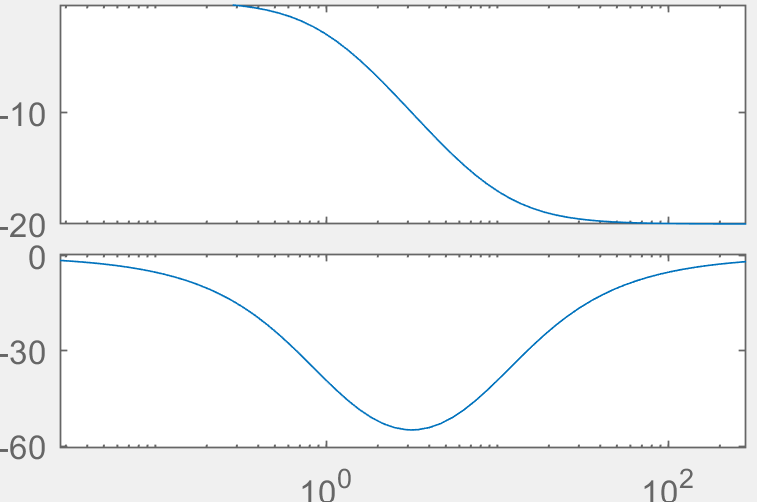
\includegraphics[width = \linewidth]{src/images/lag-controller.png}
    \end{minipage}

    Show in Bode Plot: Phase in / decreases between $\omega_1 = a$ and $\omega_2 = b$, midpoint between $b$ an $a$ is given by $\sqrt{ab}$ 

    \titel{similarities of PID and Lead / Lag compensators}
        \begin{align*}
            PID(s) = k \cdot \underbrace{\frac{\frac{s}{z_1} + 1}{s + 0}}_{\text{Lag}} \cdot \underbrace{\frac{\frac{s}{z_2} + 1}{\frac{s}{p} + 1}}_{\text{Lead}}
        \end{align*}
        p refers to a "fast pole", This is necessary for the controller to be implementable